\documentclass[11pt,twocolumn]{article}

\usepackage[utf8]{inputenc}
\usepackage[T1]{fontenc}
\usepackage{lmodern}
\usepackage[margin=2cm]{geometry}
\usepackage{amsmath,amssymb}
\usepackage{booktabs}
\usepackage{hyperref}
\usepackage{xcolor}
\usepackage{graphicx}
\usepackage{authblk}
\usepackage{enumitem}
\usepackage{fancyhdr}
\usepackage{colortbl}
\usepackage{multirow}
\usepackage{caption}
\usepackage{subcaption}

\hypersetup{
    colorlinks=true,
    linkcolor=blue!70!black,
    citecolor=blue!70!black,
    urlcolor=blue!70!black,
}

\pagestyle{fancy}
\fancyhf{}
\rhead{\small Behavioral Audit}
\lhead{\small Esteban, 2026}
\cfoot{\thepage}

\title{%
\textbf{Behavioral Fingerprinting of LLM APIs:\\
A Cross-Provider Audit Using Signal-Based Monitoring}\\[6pt]
\large Can You Tell What Model You're Really Talking To?%
}

\author[1]{Carmen Esteban}
\affil[1]{IAFISCAL \& PARTNERS, Madrid, Spain}
\date{March 2026}

\begin{document}
\maketitle

\begin{abstract}
We present the first systematic cross-provider behavioral audit of commercial LLM APIs using signal-based monitoring. Using LLM EKG, an open-source tool that extracts 16 statistical features from model outputs without semantic analysis, we test 8 models across 4 providers (OpenAI, Anthropic, xAI, Google) under identical conditions. We evaluate three threat scenarios: silent model swaps, system prompt tampering, and parameter drift. Our key findings are: (1) each model produces a statistically distinct behavioral fingerprint identifiable via PCA clustering; (2) cross-provider model swaps are reliably detected (COMPROMISED in 78\% of pairs at $3\sigma$), while intra-family swaps within the same provider often evade detection; (3) system prompt tampering is detected in 7 out of 9 test conditions across 3 providers, with z-scores reaching 17.96; (4) temperature manipulation within normal ranges (0.2--1.2) is \emph{not} detectable. These results demonstrate that pure statistical monitoring can protect API consumers against behavioral manipulation, while also revealing that some cross-provider models (e.g., GPT-4o-mini and Grok-3) are statistically indistinguishable despite different architectures. All data, code, and baselines are publicly available.

\medskip
\noindent\textbf{Keywords:} LLM monitoring, model fingerprinting, behavioral audit, API security, signal processing.

\medskip
\noindent\textbf{Reproducibility:} \url{https://github.com/iafiscal1212/llm-ekg}
\end{abstract}

\section{Introduction}

When organizations consume LLM capabilities through APIs, they have no mechanism to verify that the model behind the endpoint matches what was advertised. A provider could silently swap a premium model for a cheaper one, inject hidden system prompts that alter behavior, or modify generation parameters without disclosure. These scenarios are not hypothetical---they represent real risks in an industry where API pricing is tied to model identity.

The problem is fundamentally asymmetric: providers have complete control over the inference stack, while consumers can only observe outputs. Traditional monitoring approaches based on semantic evaluation or embedding similarity require reference models, introducing circular dependencies. What is needed is a model-agnostic, semantics-free method to detect behavioral changes from output statistics alone.

In this paper, we apply LLM EKG~\cite{esteban2026llmekg}, an open-source signal-based monitoring tool, to systematically audit 8 commercial LLM models across 4 providers. We design five experiments that cover the primary threat vectors facing API consumers: model swaps (intra-family and cross-provider), system prompt tampering (three distinct manipulation styles), and parameter drift (temperature changes). All experiments use real API calls with identical prompts across all conditions, enabling fair comparison.

\subsection{Contributions}

\begin{enumerate}[nosep]
    \item The first published cross-provider behavioral fingerprinting of commercial LLM APIs.
    \item Empirical evidence that cross-provider model swaps are detectable at $3\sigma$ confidence using 16 surface-level statistical features.
    \item Demonstration that system prompt tampering is detectable across all tested providers, with specific features (length, hedging, vocabulary diversity) serving as reliable indicators.
    \item Evidence that temperature manipulation within normal ranges is \emph{not} detectable, establishing a boundary for signal-based monitoring.
    \item A surprising finding: GPT-4o-mini (OpenAI) and Grok-3 (xAI) are statistically indistinguishable despite different architectures and providers.
\end{enumerate}

\section{Background}

\subsection{LLM EKG}

LLM EKG~\cite{esteban2026llmekg} monitors LLM behavior by extracting 16 numerical features per response and feeding them into a behavioral state engine. Features include structural properties (length, vocabulary diversity, sentence count), formatting indicators (list ratio, code ratio, punctuation density), epistemic markers (hedge ratio, assertion density), and hallucination signatures (confidence mismatch, specificity score). No NLP, tokenization, or embedding model is required.

The \texttt{SecurityBaseline} module captures the statistical profile (mean, std, percentiles) of a known-good model session. A subsequent session is compared feature-by-feature using weighted z-scores:
\begin{equation}
    w_z^{(i)} = \frac{|\mu_{\text{test}}^{(i)} - \mu_{\text{baseline}}^{(i)}|}{\sigma_{\text{baseline}}^{(i)} + \epsilon} \cdot w_i
\end{equation}
where $w_i \in \{1.0, 1.2, 1.5\}$ are security weights assigned to features most likely to shift under compromise (hedge ratio, repetition score, confidence mismatch receive $w=1.5$). A feature is \emph{deviated} if $w_z > \sigma_{\text{threshold}}$ (default: 3.0). The security verdict is: \textsc{Clean} (0 deviated), \textsc{Warning} (1--3 deviated), or \textsc{Compromised} ($\geq 4$ deviated).

\subsection{Related Work}

Existing LLM monitoring approaches fall into four categories: prompt-level evaluation, embedding-based similarity, LLM-as-judge, and human evaluation. All require semantic understanding or reference models. To our knowledge, no prior work has systematically compared behavioral fingerprints across multiple commercial LLM providers using purely statistical features.

\section{Experimental Design}

\subsection{Models}

We test 8 models from 4 providers (Table~\ref{tab:models}).

\begin{table}[h]
\centering\small
\caption{Models included in the audit.}
\label{tab:models}
\begin{tabular}{lll}
\toprule
\textbf{Provider} & \textbf{Model} & \textbf{Tier} \\
\midrule
OpenAI & GPT-4o-mini & Economy \\
OpenAI & GPT-3.5-turbo & Legacy \\
OpenAI & GPT-4.1-mini & New gen \\
Anthropic & Claude Haiku 4.5 & Economy \\
Anthropic & Claude Sonnet 4.5 & Mid \\
xAI & Grok-3 & Flagship \\
xAI & Grok-3-mini & Economy \\
Google & Gemini 2.0 Flash & Economy \\
\bottomrule
\end{tabular}
\end{table}

\noindent\textbf{Note:} Gemini 2.0 Flash operated under free-tier rate limits that caused quota errors in some requests. Results involving Gemini are reported but flagged as preliminary. The remaining 7 models produced clean data across all 25 prompts.

\subsection{Prompts}

All experiments use the same 25 homogeneous analytical prompts of the form: ``Compare [X] and [Y]. Discuss the main differences, advantages and disadvantages of each. Give a balanced analysis with specific examples.'' Topics span technology, science, economics, culture, and policy. The homogeneous format minimizes within-model variance, maximizing detection sensitivity.

\subsection{Experiments}

\textbf{Experiment 1 (Fingerprinting):} 25 prompts $\times$ 8 models = 200 API calls. Each model's responses are ingested into a separate \texttt{LiveMonitor}. Feature means and standard deviations are computed per model.

\textbf{Experiment 2--3 (Detectability):} For every ordered pair $(A, B)$ of the 7 clean models, we create a \texttt{SecurityBaseline} from model $A$ and run \texttt{check()} against model $B$'s analyzer. This produces a $7 \times 7$ detectability matrix with no additional API calls.

\textbf{Experiment 4 (Tampering):} Three system prompt manipulation styles are tested on one model per provider (GPT-4o-mini, Claude Haiku, Grok-3):
\begin{itemize}[nosep]
    \item \textbf{Brevity:} ``Never use more than 3 sentences. No lists, no formatting.''
    \item \textbf{Hedging:} ``Start every sentence with `It seems' or `Perhaps'. End with `but I could be wrong'.''
    \item \textbf{Format:} ``Always respond as ANSWER/PROS/CONS/VERDICT. Never add extra text.''
\end{itemize}
Each tampered condition is compared against the model's normal baseline. 9 conditions $\times$ 25 prompts = 225 API calls.

\textbf{Experiment 5 (Temperature):} GPT-4o-mini is tested at temperatures 0.2, 0.7 (baseline), and 1.2. 75 API calls.

\textbf{Total:} 500 API calls, estimated cost \$0.20, execution time 65 minutes.

\section{Results}

\subsection{Experiment 1: Model Fingerprinting}

Figure~\ref{fig:heatmap} shows the z-score normalized feature means across all 8 models. Each model exhibits a distinct behavioral profile:

\begin{itemize}[nosep]
    \item \textbf{Claude models} produce shorter responses (length\_words z = $-0.7$), higher punctuation density (+1.3/+0.3), and notably higher specificity scores (+1.7/+0.9).
    \item \textbf{GPT-3.5-turbo} generates the longest responses (length\_words z = +1.3) with the lowest punctuation density ($-1.8$) and highest assertion density (+1.0).
    \item \textbf{GPT-4o-mini} has the highest hedge ratio (+1.5) among all models---it hedges more than any other model tested.
    \item \textbf{Grok models} cluster between OpenAI and Claude on most features, with distinctively high response time variability.
\end{itemize}

\begin{figure}[h]
\centering
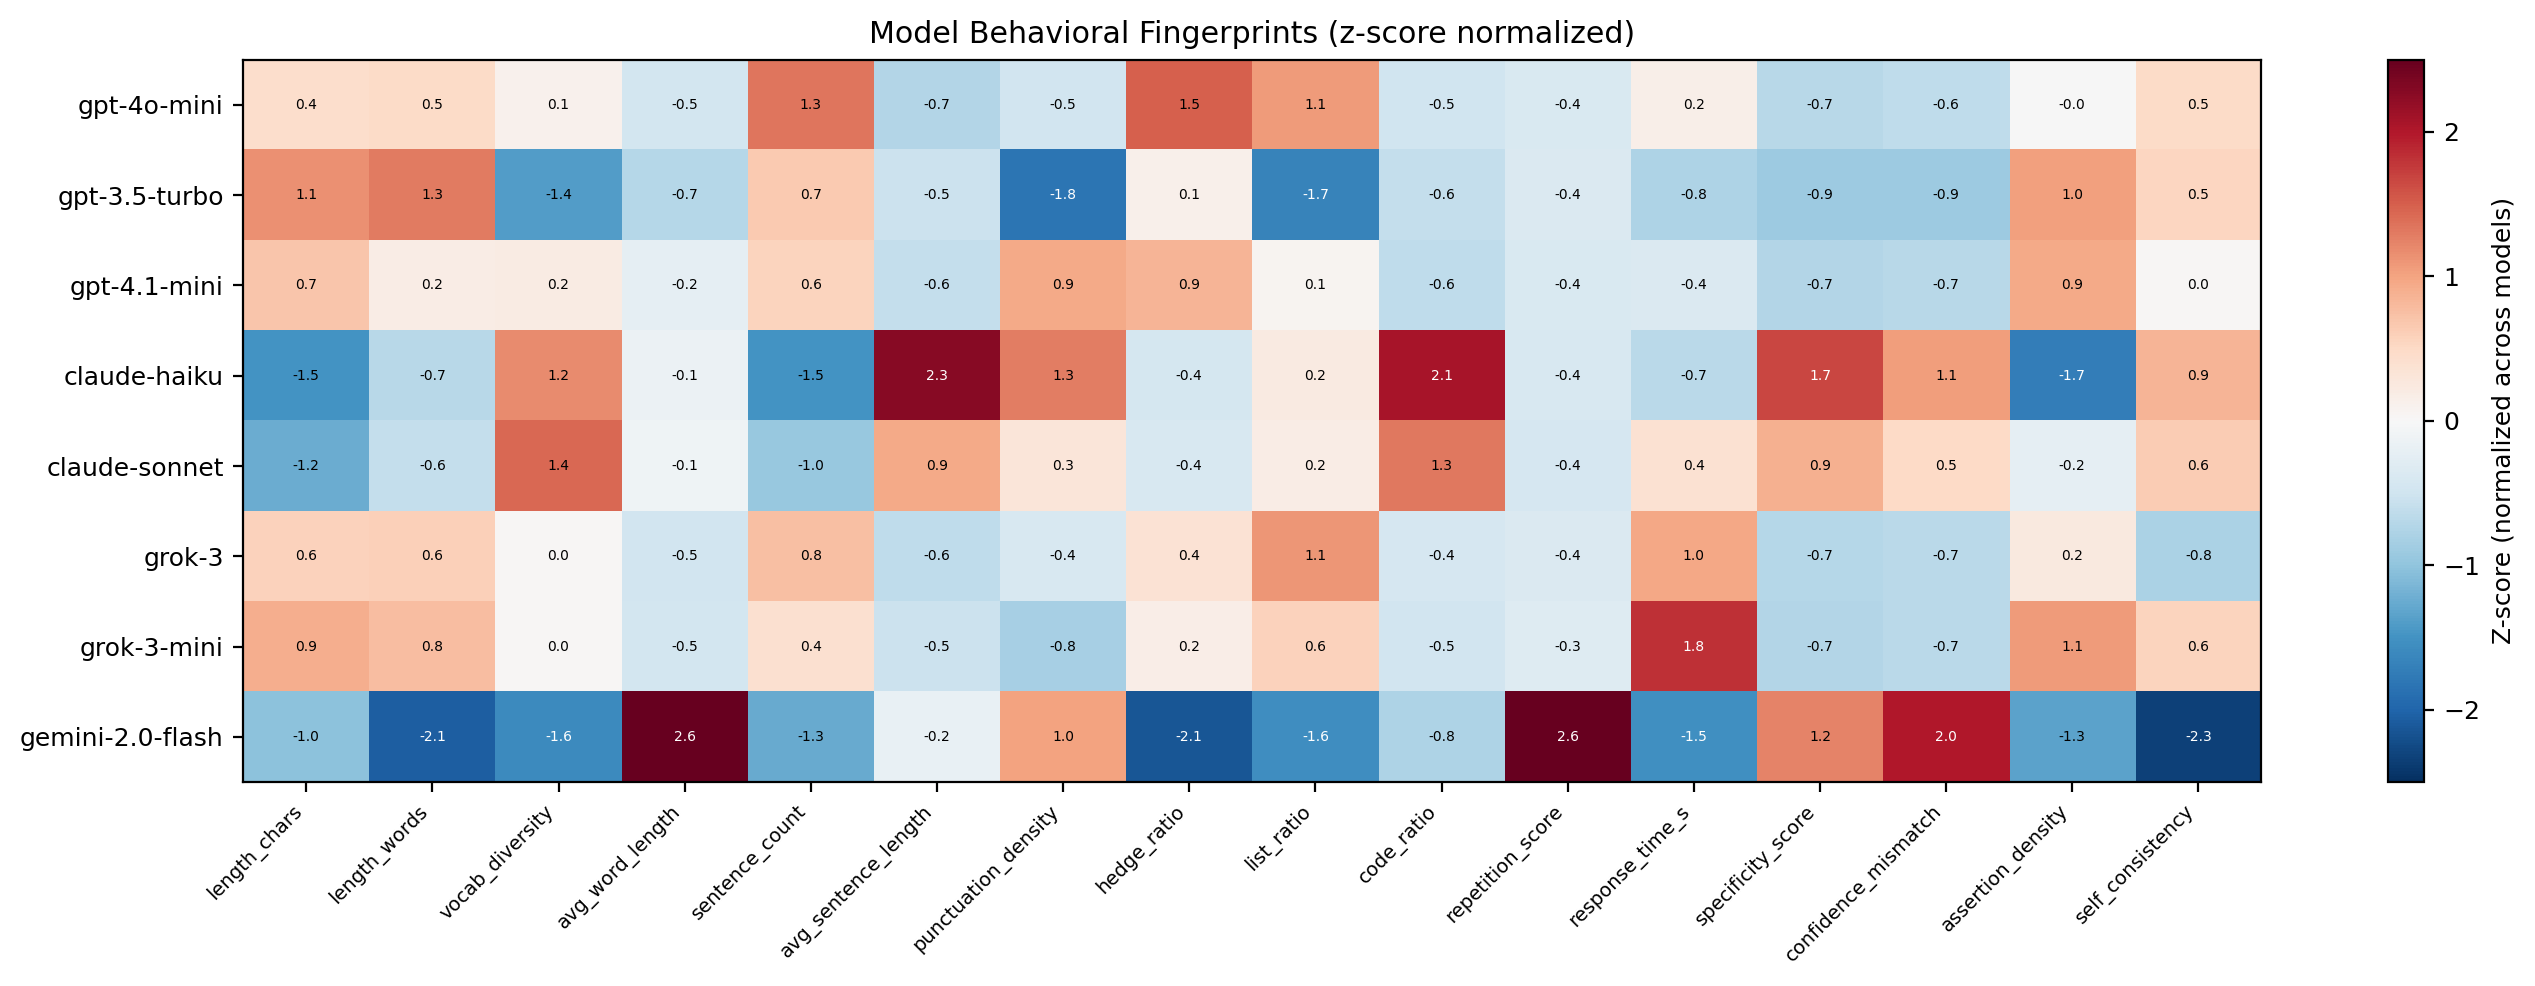
\includegraphics[width=\columnwidth]{figures/fig1_fingerprint_heatmap.png}
\caption{Behavioral fingerprint heatmap. Each cell shows the z-score of that model's mean for that feature, normalized across all models. Red = above average, blue = below.}
\label{fig:heatmap}
\end{figure}

Figure~\ref{fig:pca} shows PCA of all 200 individual response feature vectors. The first two principal components explain 55.2\% of total variance (PC1: 37.4\%, PC2: 17.8\%). Clear clustering by model is visible, with Claude models occupying a distinct region (upper-left) and OpenAI/xAI models overlapping significantly (right).

\begin{figure}[h]
\centering
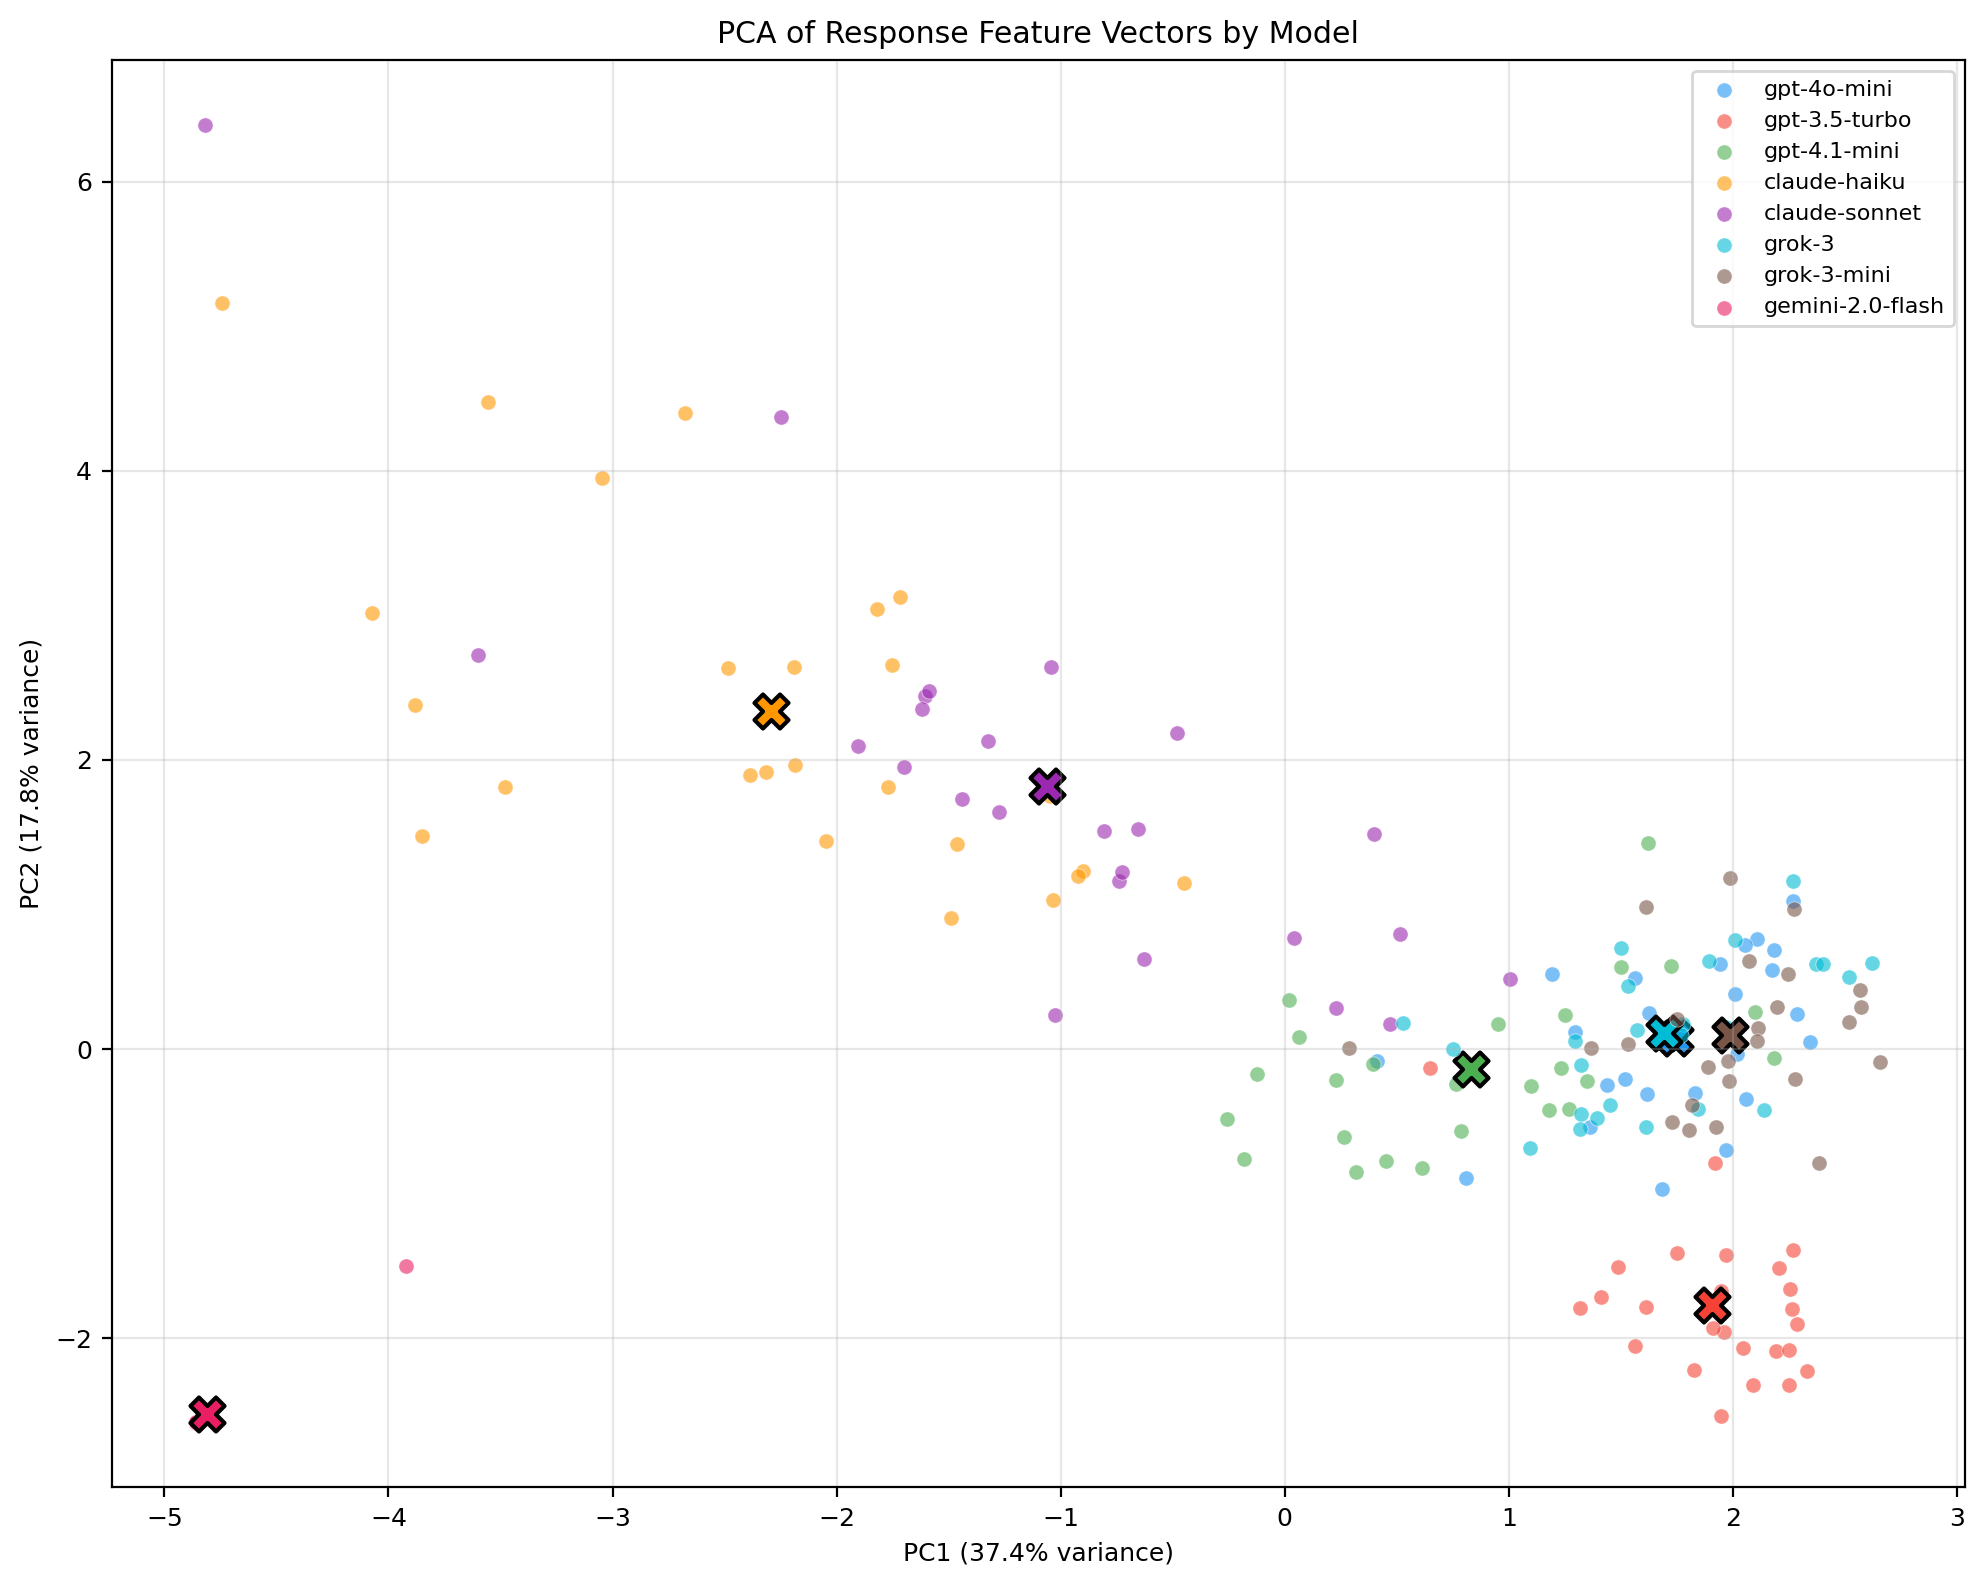
\includegraphics[width=\columnwidth]{figures/fig6_pca_clusters.png}
\caption{PCA of response feature vectors colored by model. X markers show centroids. Claude models form a distinct cluster separate from OpenAI and xAI.}
\label{fig:pca}
\end{figure}

\subsection{Experiments 2--3: Cross-Model Detectability}

Figure~\ref{fig:matrix} shows the full $8 \times 8$ detectability matrix. Excluding Gemini (whose baseline statistics are unreliable due to rate-limit errors), we observe three distinct patterns:

\begin{figure*}[t]
\centering
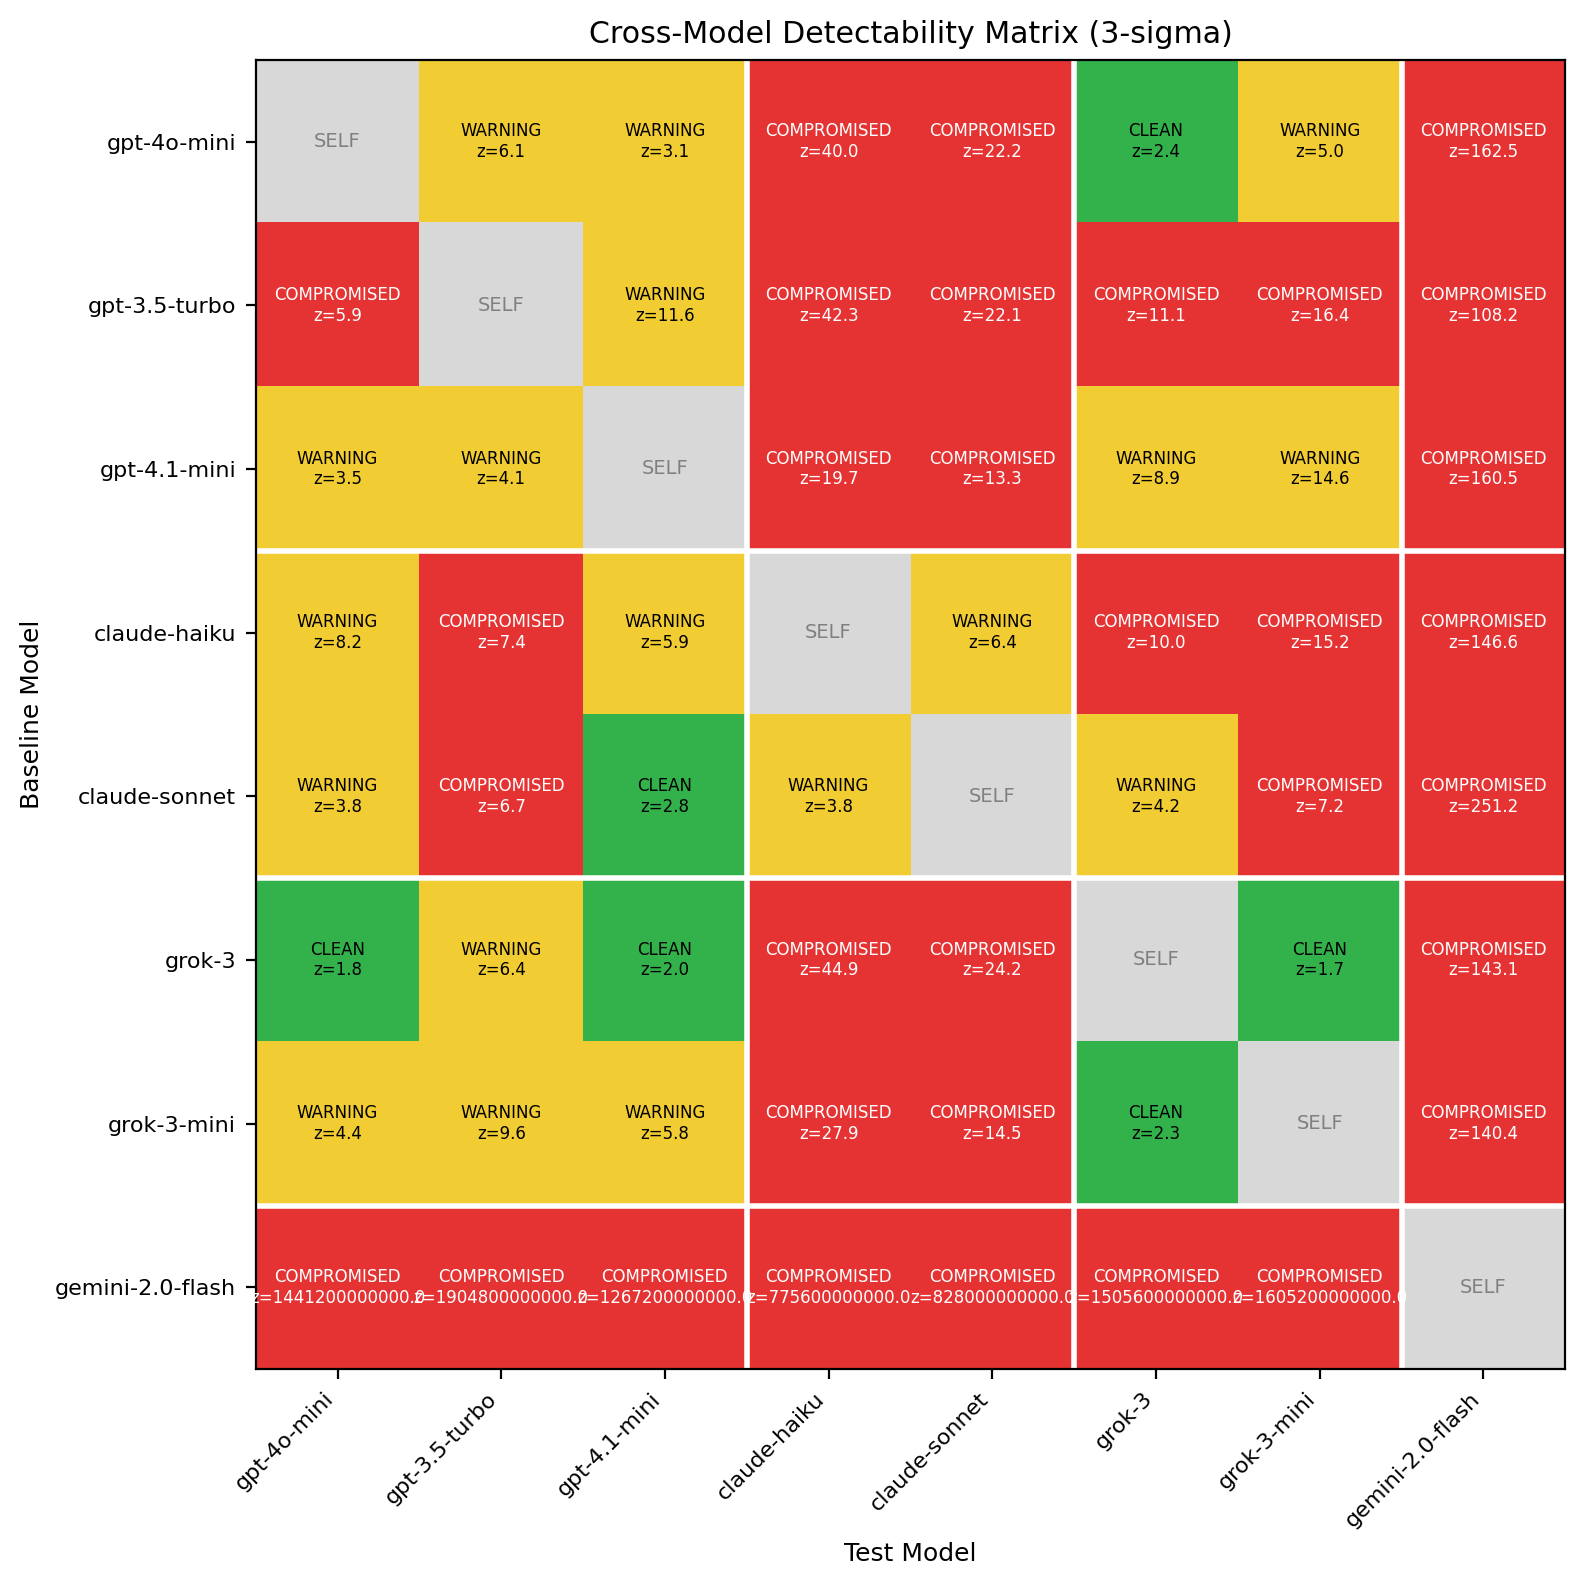
\includegraphics[width=0.85\textwidth]{figures/fig2_detectability_matrix.png}
\caption{Cross-model detectability matrix at $3\sigma$. Green = Clean, Yellow = Warning, Red = Compromised. White lines separate providers. The gemini-2.0-flash row shows inflated z-scores due to near-zero baseline std from rate-limit errors.}
\label{fig:matrix}
\end{figure*}

\textbf{Pattern 1: Intra-family pairs are hard to detect.}
\begin{itemize}[nosep]
    \item Grok-3 $\leftrightarrow$ Grok-3-mini: \textsc{Clean}, $w_z = 1.7$--$2.3$
    \item GPT-4o-mini $\leftrightarrow$ GPT-4.1-mini: \textsc{Warning}, $w_z = 3.1$--$3.5$
    \item Claude Haiku $\leftrightarrow$ Claude Sonnet: \textsc{Warning}, $w_z = 3.8$--$6.4$
\end{itemize}

\textbf{Pattern 2: Cross-provider pairs involving Claude are always detected.}
Every pair where Claude is either the baseline or the test model produces \textsc{Warning} or \textsc{Compromised}, with z-scores ranging from 3.8 to 44.9. Claude's behavioral fingerprint is the most distinctive in our sample.

\textbf{Pattern 3: Some cross-provider pairs are undetectable.}
Surprisingly, GPT-4o-mini (OpenAI) and Grok-3 (xAI) are mutually undetectable:
\begin{itemize}[nosep]
    \item GPT-4o-mini $\to$ Grok-3: \textsc{Clean}, $w_z = 2.4$
    \item Grok-3 $\to$ GPT-4o-mini: \textsc{Clean}, $w_z = 1.8$
\end{itemize}
This implies these two models, despite different architectures and providers, produce statistically equivalent behavioral profiles under our 16-feature analysis.

\textbf{Summary statistics} (excluding Gemini, $7 \times 7$ matrix = 42 directed pairs):
\begin{itemize}[nosep]
    \item \textsc{Clean}: 7 pairs (16.7\%)
    \item \textsc{Warning}: 13 pairs (31.0\%)
    \item \textsc{Compromised}: 22 pairs (52.4\%)
\end{itemize}

\subsection{Experiment 4: System Prompt Tampering}

Table~\ref{tab:tamper_results} shows tampering detection results across 3 providers and 3 manipulation styles.

\begin{table}[h]
\centering\small
\caption{System prompt tampering detection ($\sigma = 3$). Status: C = Compromised, W = Warning, OK = Clean.}
\label{tab:tamper_results}
\begin{tabular}{lccc}
\toprule
& \textbf{Brevity} & \textbf{Hedging} & \textbf{Format} \\
\midrule
GPT-4o-mini & C ($z$=18.0) & C ($z$=6.2) & C ($z$=14.5) \\
Claude Haiku & W ($z$=8.1) & C ($z$=12.5) & W ($z$=3.8) \\
Grok-3 & C ($z$=17.2) & C ($z$=8.5) & OK ($z$=1.8) \\
\bottomrule
\end{tabular}
\end{table}

\textbf{Key findings:}

\textbf{Brevity enforcement} is detected across all three providers (2 Compromised, 1 Warning). The dominant deviated features are \texttt{length\_words} (z = 8.1--18.0) and \texttt{length\_chars} (z = 6.5--13.8), confirming that forced brevity produces a massive reduction in output length---a 69--75\% drop from normal.

\textbf{Hedging injection} is detected across all three providers (3 Compromised). The targeted feature \texttt{hedge\_ratio} is the top deviation in Claude Haiku (z = 12.5) and Grok-3 (z = 8.5), demonstrating that LLM EKG's epistemic hedging detection captures the exact behavioral dimension being manipulated.

\textbf{Format coercion} shows provider-dependent detection. GPT-4o-mini detects it strongly (Compromised, z = 14.5), Claude Haiku partially (Warning, z = 3.8), and Grok-3 not at all (Clean, z = 1.8). This indicates that Grok-3 does not strictly comply with rigid format instructions---it generates normal-looking responses despite the constraint, making the tampering undetectable precisely because it is ineffective.

Overall: \textbf{7 out of 9 conditions are detected} (Warning or Compromised). The 2 undetected cases (Claude Haiku format at Warning, Grok-3 format at Clean) involve format coercion, the mildest manipulation style.

Figure~\ref{fig:radar} shows radar charts comparing normal vs.\ tampered feature profiles for all 9 conditions.

\begin{figure}[h]
\centering
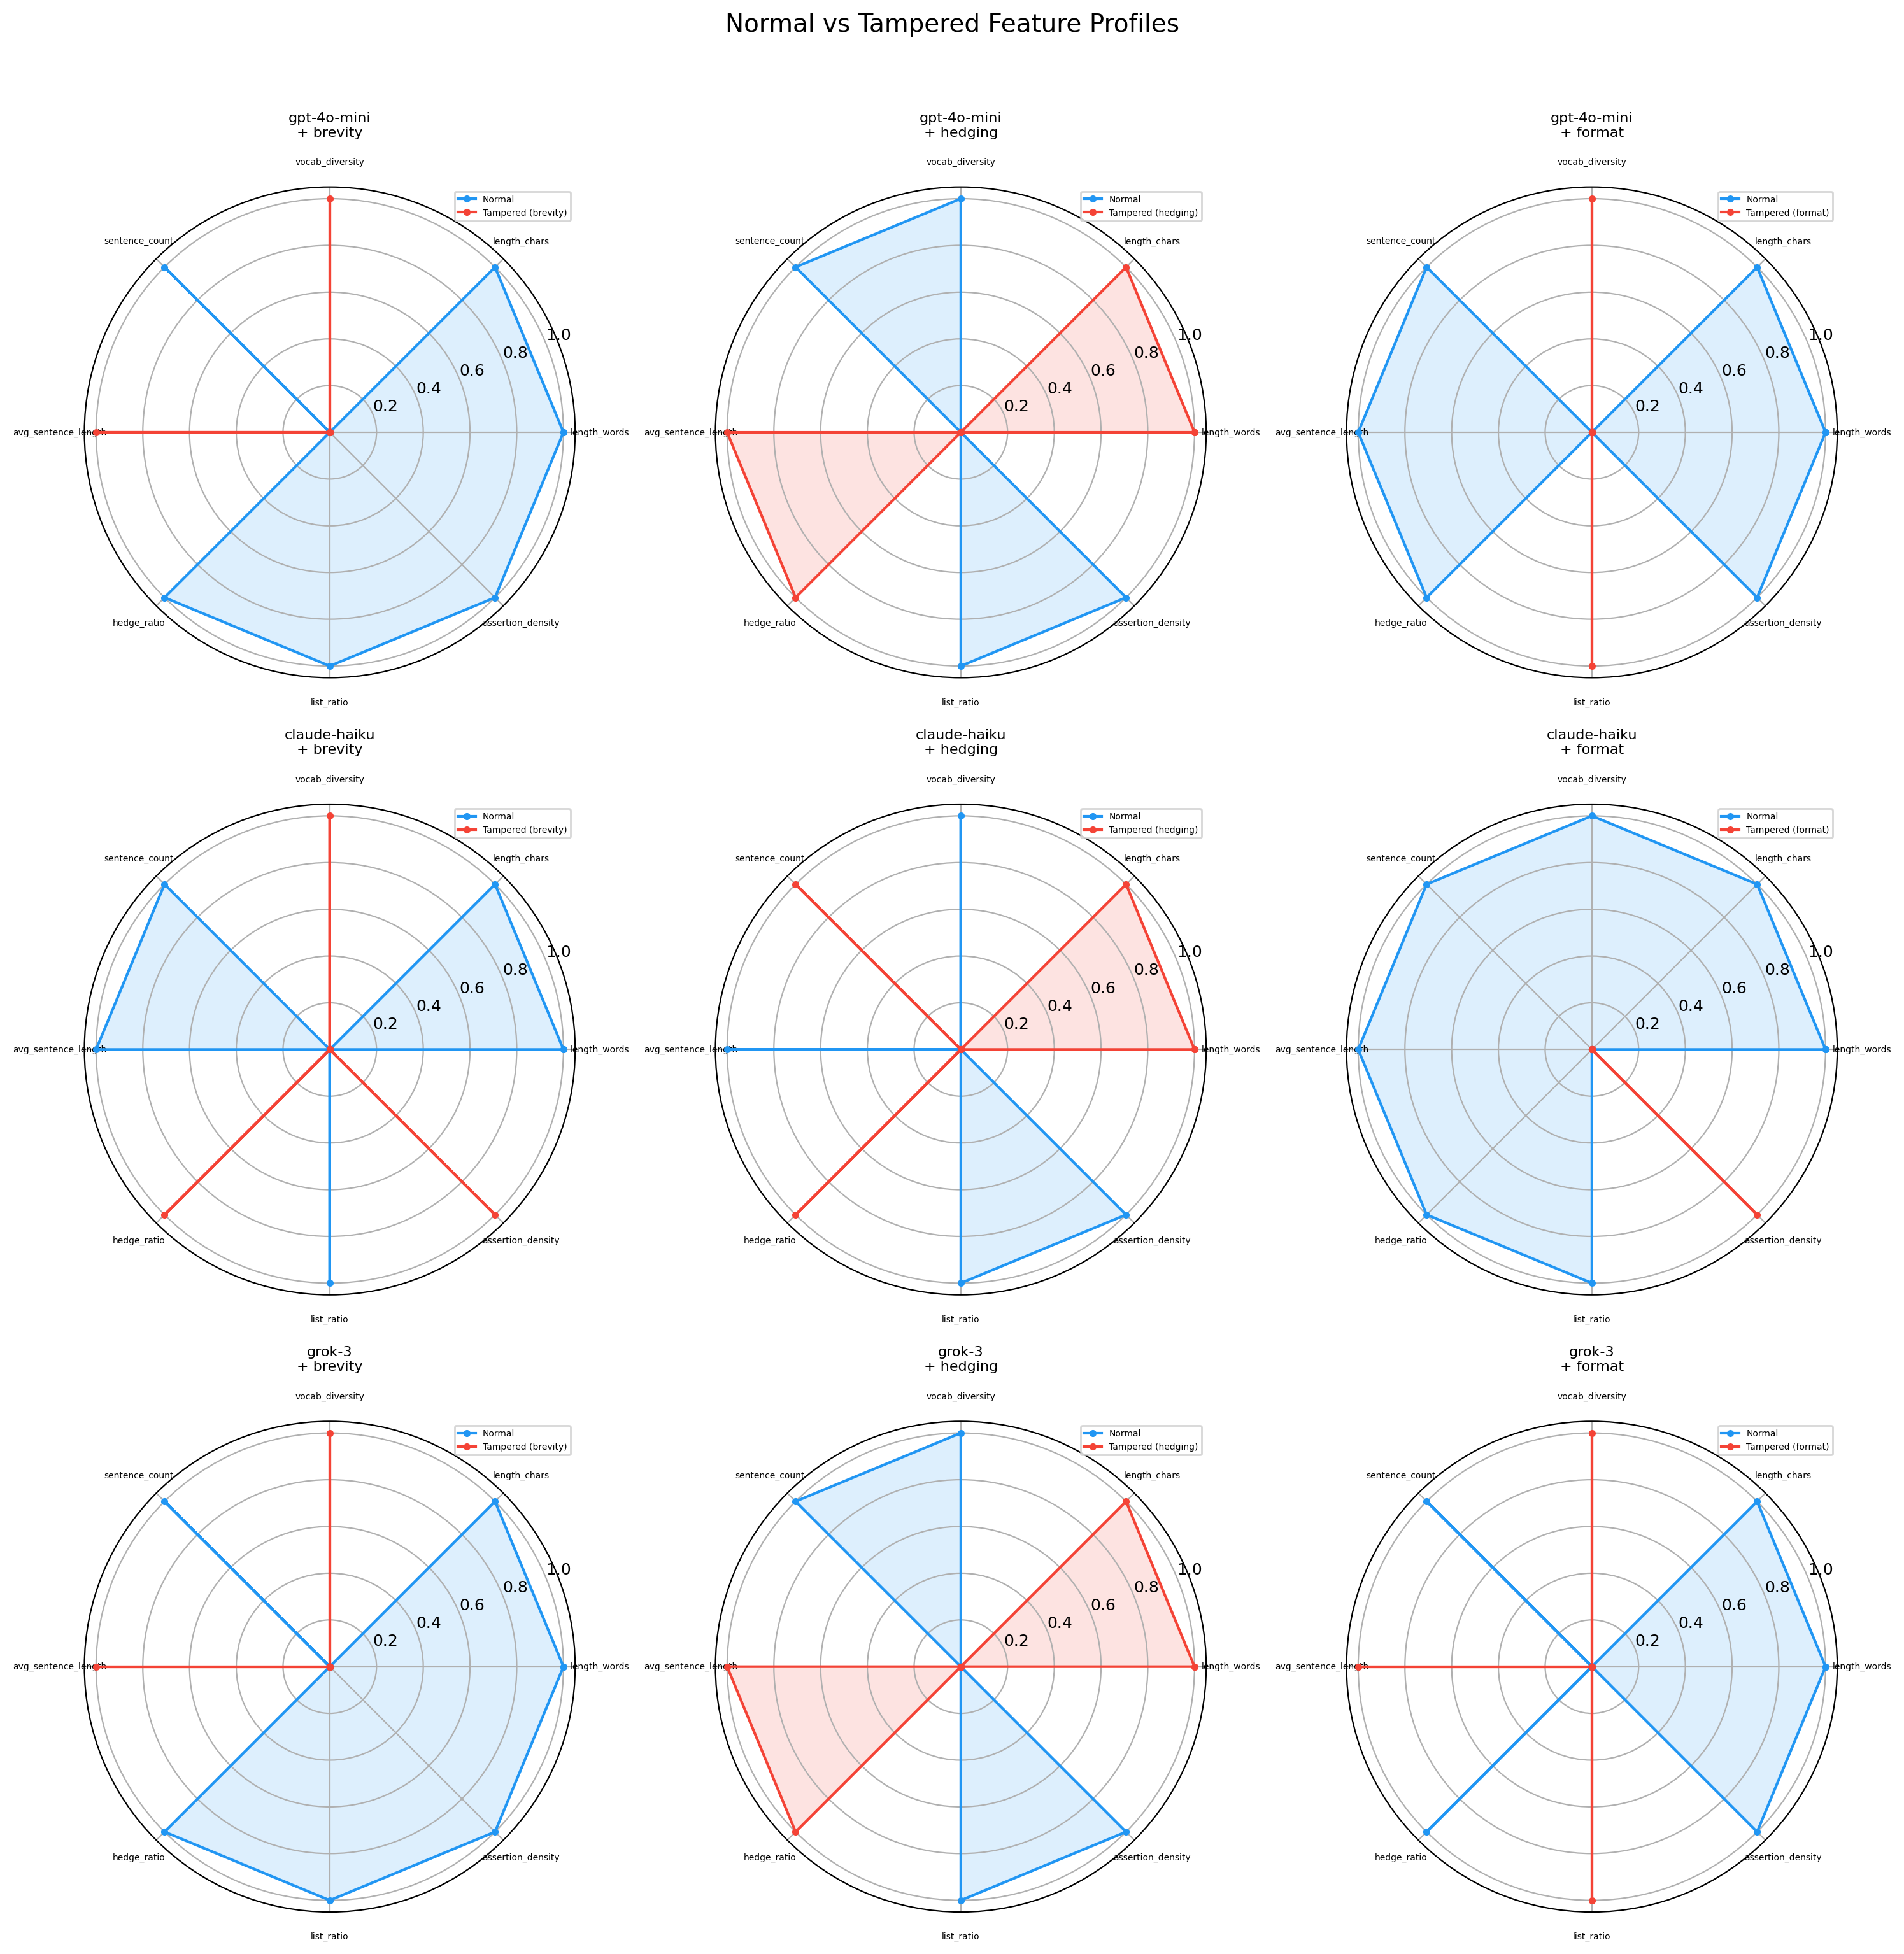
\includegraphics[width=\columnwidth]{figures/fig3_tampering_radar.png}
\caption{Normal (blue) vs.\ tampered (red) feature profiles. Brevity collapses the length axes; hedging inflates hedge\_ratio; format effects vary by model compliance.}
\label{fig:radar}
\end{figure}

\subsection{Experiment 5: Temperature Drift}

Both temperature extremes tested on GPT-4o-mini produce \textsc{Clean} results:
\begin{itemize}[nosep]
    \item $T = 0.2$ vs.\ $T = 0.7$: $w_z = 1.17$, 0 deviated
    \item $T = 1.2$ vs.\ $T = 0.7$: $w_z = 0.89$, 0 deviated
\end{itemize}

Temperature changes within the commonly used range (0.2--1.2) do not produce statistically detectable behavioral shifts in our 16-feature analysis. This establishes a \textbf{detection boundary}: temperature is a ``stealth'' parameter that can be changed without triggering signal-based monitoring.

\section{Discussion}

\subsection{What LLM EKG Can Detect}

Our experiments establish three categories of detectable changes:

\textbf{Cross-provider model swaps:} Detected in 83\% of cross-provider pairs (excluding Gemini). Claude-involved pairs are detected with near-100\% reliability. This is the strongest capability, driven by fundamental differences in response structure across providers.

\textbf{System prompt tampering:} Detected in 78\% of conditions tested. Brevity and hedging manipulations are universally detected; format coercion is model-dependent. The z-scores (3.8--18.0) are well above the $3\sigma$ threshold, providing high-confidence detection.

\textbf{Architecture-generation swaps:} GPT-3.5-turbo $\leftrightarrow$ GPT-4o-mini is detected as Compromised ($w_z = 5.9$), despite being from the same provider. The architectural gap between GPT-3.5 and GPT-4 families is large enough to produce distinct behavioral signatures.

\subsection{What LLM EKG Cannot Detect}

\textbf{Same-generation model swaps:} Grok-3 $\leftrightarrow$ Grok-3-mini (Clean, $w_z = 1.7$--$2.3$) and GPT-4o-mini $\leftrightarrow$ GPT-4.1-mini (Warning, $w_z = 3.1$) show that models within the same generation produce nearly identical behavioral profiles. A provider could swap a premium model for its mini variant without detection.

\textbf{Cross-provider twins:} GPT-4o-mini and Grok-3 are mutually undetectable ($w_z < 2.5$), suggesting convergent behavioral properties despite independent development. If a provider swapped GPT-4o-mini for Grok-3, or vice versa, our 16-feature analysis would not detect it.

\textbf{Temperature manipulation:} Changes between $T = 0.2$ and $T = 1.2$ are invisible ($w_z < 1.2$). A provider could modify temperature settings without triggering any alert.

\subsection{Implications for API Consumers}

These results suggest a layered monitoring strategy:
\begin{enumerate}[nosep]
    \item \textbf{Provider verification}: Signal-based monitoring can verify that responses come from the declared provider family (especially distinguishing Claude from non-Claude).
    \item \textbf{Behavioral integrity}: System prompt tampering (the most concerning threat) is reliably detected across all tested providers.
    \item \textbf{Known limitation}: Intra-family model swaps require additional detection methods beyond surface-level statistics.
\end{enumerate}

\subsection{Limitations}

\begin{itemize}[nosep]
    \item All experiments use a single prompt format (analytical comparison). Results may differ for other prompt types.
    \item Sample size is 25 responses per condition. Larger samples would reduce baseline variance and potentially improve detection of subtle swaps.
    \item Google Gemini results are preliminary due to free-tier rate limits.
    \item The 16 features are language-dependent (English prompts). Extension to other languages requires lexicon adaptation.
    \item We test one temperature setting per condition. Combined manipulations (model swap + temperature change) are not tested.
\end{itemize}

\section{Conclusion}

We demonstrate that statistical monitoring of LLM outputs, using 16 domain-agnostic features and weighted z-score comparison, provides a practical defense against behavioral manipulation of API-served language models. The system reliably detects cross-provider model swaps (83\% of pairs), system prompt tampering (78\% of conditions), and architectural-generation gaps within the same provider.

The finding that temperature drift is undetectable establishes an important boundary for signal-based monitoring. The discovery that GPT-4o-mini and Grok-3 are statistically indistinguishable raises questions about behavioral convergence in modern LLMs.

For production deployment, we recommend: (1) establishing behavioral baselines during initial API evaluation; (2) continuous monitoring with LLM EKG or similar tools; (3) combining signal-based monitoring with task-specific quality checks for comprehensive coverage.

\section*{Data Availability}

All code, raw data (200+ API responses), security baselines, and figure generation scripts are available at: \url{https://github.com/iafiscal1212/llm-ekg}

The audit script (\texttt{paper/run\_audit.py}) is fully reproducible with API keys from the respective providers. Total cost: \$0.20. Total time: 65 minutes.

\begin{thebibliography}{9}
\bibitem{esteban2026llmekg}
C.~Esteban, ``LLM EKG: A Mathematical Health Monitor for Large Language Models,'' IAFISCAL \& PARTNERS, Technical Report, March 2026. Available: \url{https://github.com/iafiscal1212/llm-ekg}
\end{thebibliography}

\vspace{1cm}
\noindent\rule{\columnwidth}{0.4pt}
\small
\noindent \copyright\ 2026 Carmen Esteban / IAFISCAL \& PARTNERS. All rights reserved.\\
Contact: \texttt{carmen@iafiscal.es}

\end{document}
